\documentclass[addpoints]{exam}
  % Read in shared preamble for all homeworks
  %%%%%%%%%%%%%%%%%%%%%%%%%%%%%%%%%%%%%%%%%%%%%%%%%%%%%%%%%%%%%%%%%%%%
% This is the standard preamble for homework assignments and exams %
%                                                                  %
% -Joshua McNeill (joshua dot mcneill at uga dot edu)              %
%%%%%%%%%%%%%%%%%%%%%%%%%%%%%%%%%%%%%%%%%%%%%%%%%%%%%%%%%%%%%%%%%%%%
% Exam settings
\pointsinmargin
\pointformat{}

% Packages and settings
\usepackage{fontspec}
  \setmainfont{Charis SIL}
\usepackage{tikz}

%% Custom commands
% Instructions for a section
\newcommand{\instr}[1]{
  \begin{center}
    \fbox{
      \parbox{0.85\textwidth}
             {#1}
    }
  \end{center}
}
\newcommand{\lexi}[1]{\textit{#1}}
\newcommand{\gloss}[1]{`#1'}


  % Packages and settings
  \usepackage{listings}
    \lstset{basicstyle=\ttfamily\small,
            breaklines=true}
    \usepackage{graphicx}
      \graphicspath{{../figures/}}

  % Document information
  \title{Homework 4: Psycholinguistics, Language Variation, \& Computational Linguistics}
  \date{}

\begin{document}
  \maketitle

  % Header
  %%%%%%%%%%%%%%%%%%%%%%%%%%%%%%%%%%%%%%%%%%%%%%%%%%%%%%%%%%%%%%%%%%%%%%%
% This is the the header that all homework assignments and exams use. %
%                                                                     %
% -Joshua McNeill (joshua dot mcneill at uga dot edu)                 %
%%%%%%%%%%%%%%%%%%%%%%%%%%%%%%%%%%%%%%%%%%%%%%%%%%%%%%%%%%%%%%%%%%%%%%%
\noindent\makebox[0.5\textwidth][l]{Name:} \makebox[0.5\textwidth][r]{Course: LING2100, The Study of Language}\\
\makebox[0.5\textwidth][l]{Date:} \makebox[0.5\textwidth][r]{Instructor: Joshua McNeill}


    \section{Psycholinguistics}
      \instr{On the diagram below of the left hemisphere of the cerebrum, circle and label each of the following language centers: \emph{Wernicke's area}, \emph{Broca's} area, the \emph{Angular gyrus}, and the \emph{Sylvian fissure}. (1 point each)}
  \begin{questions}
        \question[4]
          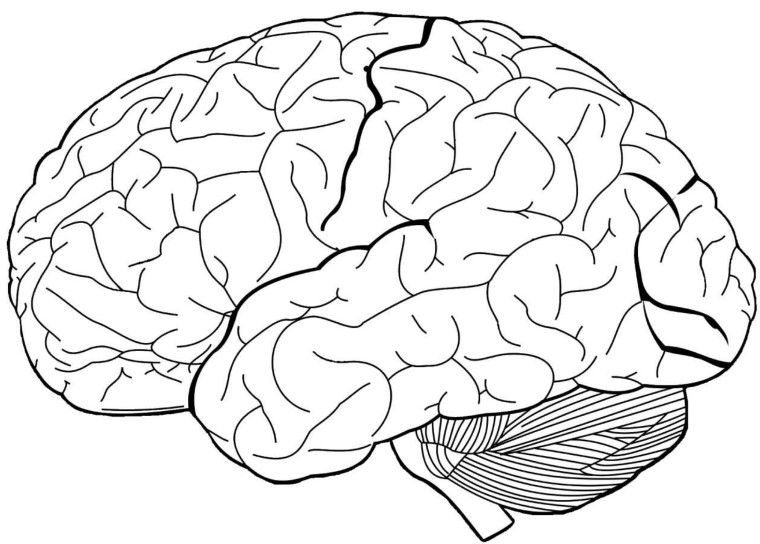
\includegraphics{brain_unlabelled.jpg}

      \newpage

      \instr{Each of the following represents speech produced by someone who suffers from either \emph{Wernicke's} aphasia or \emph{Broca's} phasia. For each, identify which type they have. (1 point each)}
        \question[1] \rule{4cm}{0.4pt} `What ... hovercraft? Well, it ... specialized boat ... sense. I mean, it go ... surface ... water. ... hovercraft ... sort of vessel ... got ... skirt all around ...'
        \question[1] \rule{4cm}{0.4pt} `I take ... thing ... down, I not put ... back. I say ... rings ... top drawer ... bureau garage. You go ... them, ... Paul ... help you ... remount ... whole thing.'
        \question[1] \rule{4cm}{0.4pt} `Now, you will infuriate from your point of percussionist that the Peruvian will be about half unlined. It will be more than that, I would think. So, you will module part of the shallow right.'
        \question[1] \rule{4cm}{0.4pt} `That right. ... tapes and conversation detail ... become ... anonymous ... completely. No one ... know who ... words ... whose voices ... tapes. Together, they ... permanent record ... English language ... speak ... number.'
        \question[1] \rule{4cm}{0.4pt} `I can't Amazonian the education window, with their shallow of money, brushing for transport for children out here to shape to the hospital to inflict a garden. The education Philson and the bogeyman governors have no desolate at all to fidget for that.'

      \instr{Each of the following represents a sentence followed by an utterance of that sentence that has an error in it. Identify the type of error being made. (1 point each)}
        \question[1] \rule{4cm}{0.4pt} \textit{Bacon and eggs} $\rightarrow$ `Beggs'
        \question[1] \rule{4cm}{0.4pt} \textit{Tom came to the barn every day} $\rightarrow$ `Tarm came to the barn every day'
        \question[1] \rule{4cm}{0.4pt} \textit{Get on the bus} $\rightarrow$ `Bet on the Gus'
        \question[1] \rule{4cm}{0.4pt} \textit{The other darts look sharp} $\rightarrow$ `The other dart look sharp'
        \question[1] \rule{4cm}{0.4pt} \textit{They rode elephants across the Alps} $\rightarrow$ `They rode Alps across the elephants'
        \question[1] \rule{4cm}{0.4pt} \textit{The struggle to survive in hostile surroundings} $\rightarrow$ `The struggles to survive in \rule{4cm}{0pt} hostile surrounding'
        \question[1] \rule{4cm}{0.4pt} \textit{Shut the back gate} $\rightarrow$ `Shut the shack gate'

      \parbox{0.6\linewidth}{
        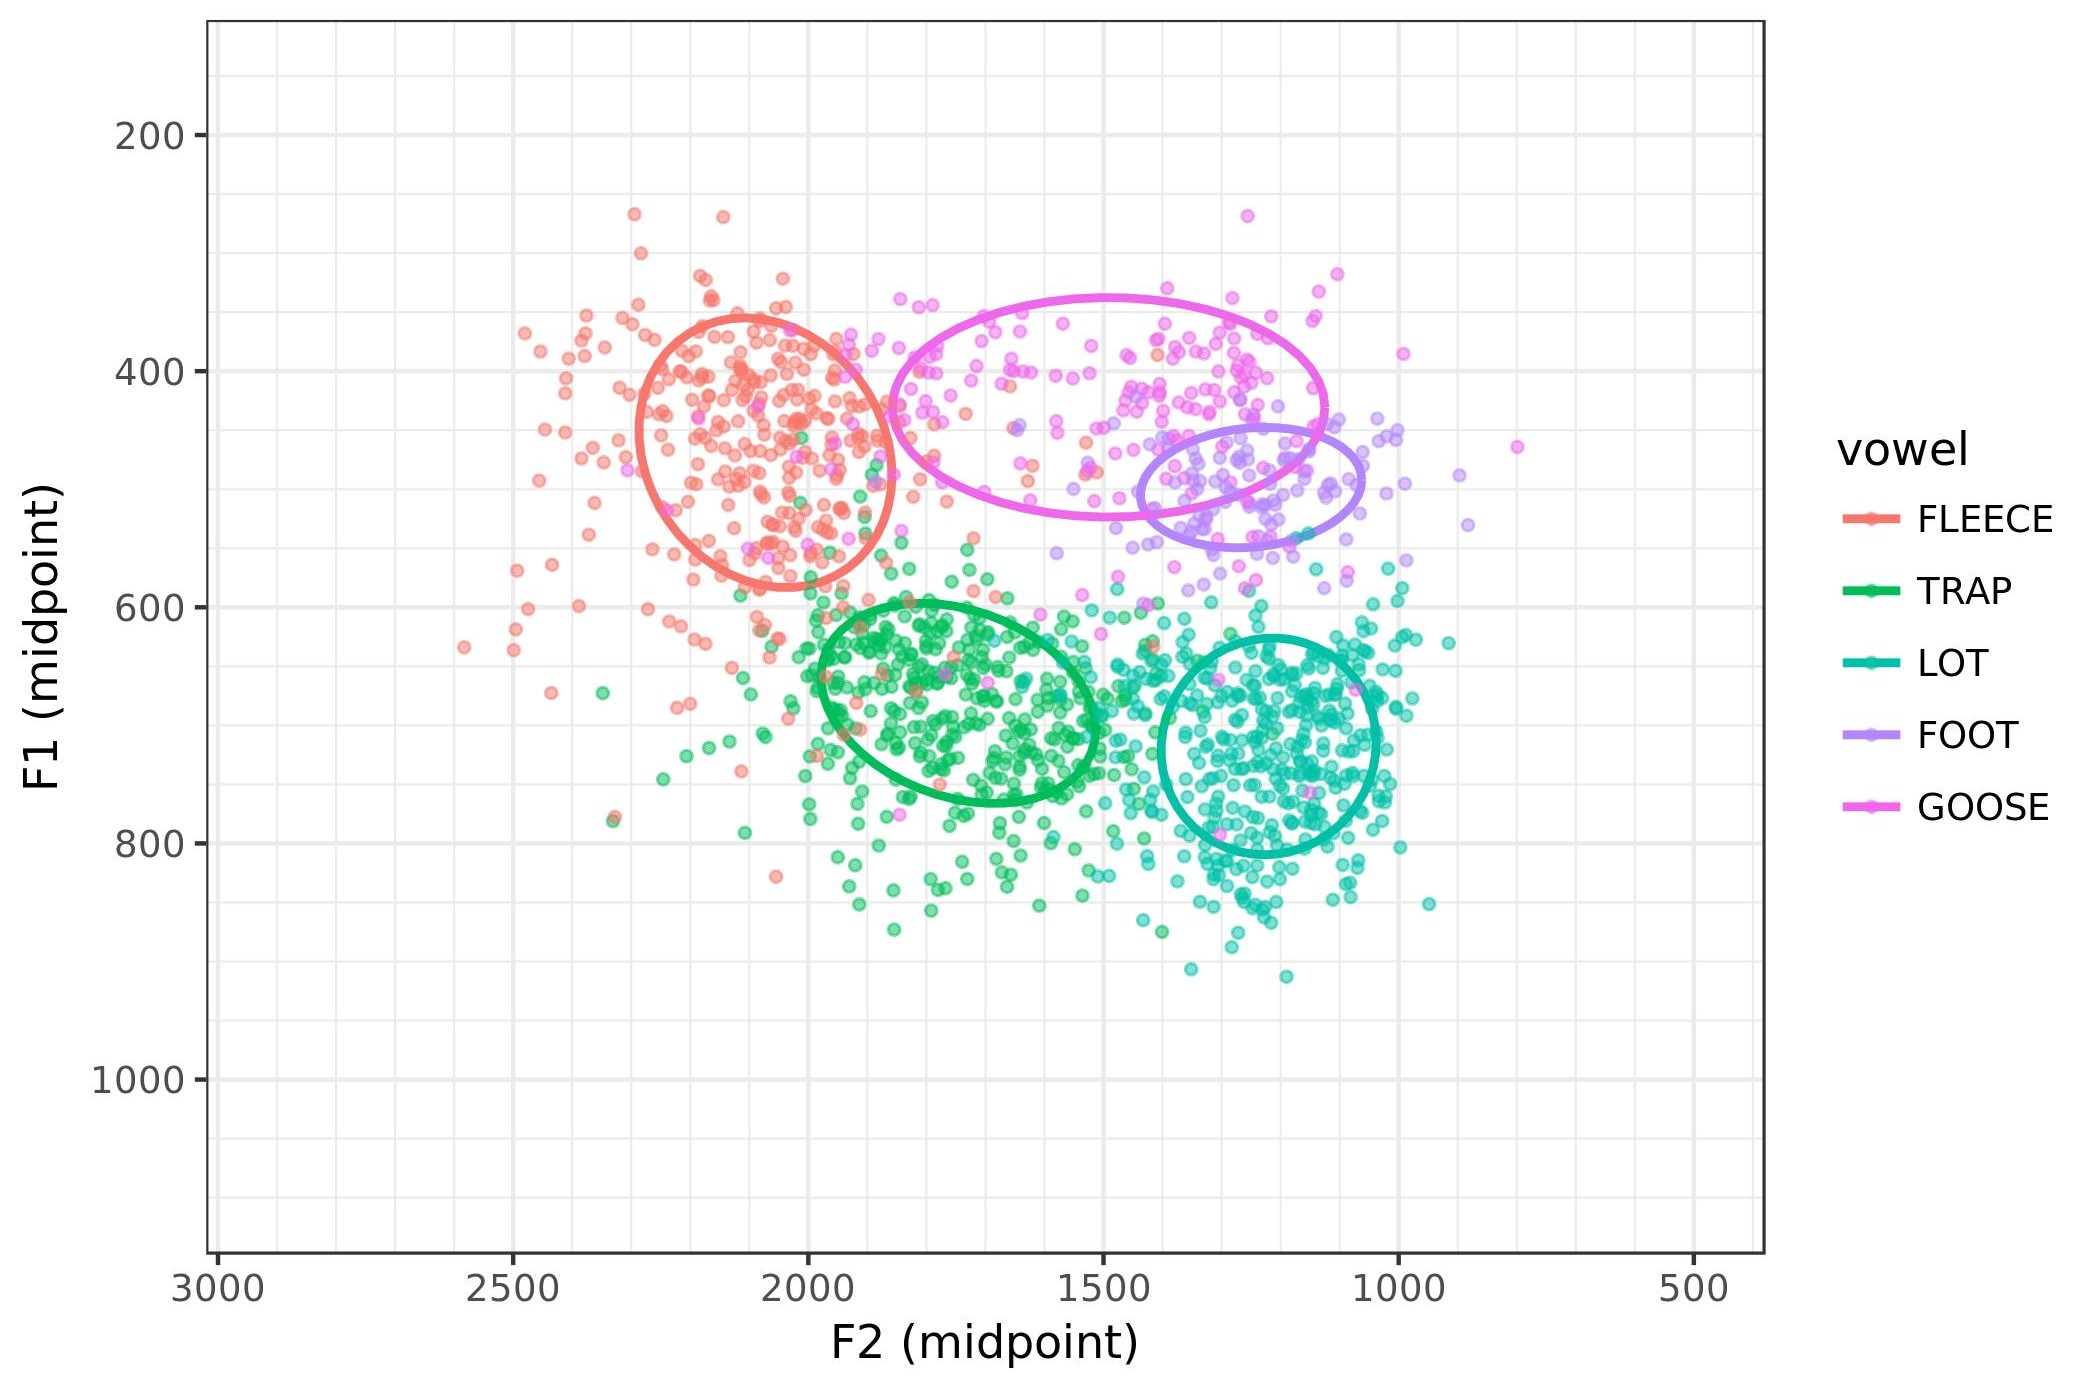
\includegraphics[scale=0.25]{vowel_perception.jpg}
      }
      \parbox{0.4\linewidth}{
        \fbox{\parbox{0.85\linewidth}{
        The chart on the left is a vowel plot where each dot represents a vowel that was produced by a speaker from Georgia. The legend gives words that are each meant to represent a specific vowel (e.g., \textit{fleece} represents the [i] vowel). Each dot on the chart represents an occurrence of the vowel that matches the dot's color. Imagine the chart represents the sort of variation that you hear when you listen to people speak and use it to answer the questions below. (1 point each)
        }}
      }

      \question[1] How many categories of vowels does your brain perceive if this data represents all the vowels you hear spoken? \hrulefill
      \question[1] How many combinations of F1 and F2 frequencies are actually produced for each category (\emph{Hint}: estimate)? \hrulefill

    \section{Language Variation}
      \instr{Many speakers in the South have what is called the \textsc{pin-pen} merger, which is the merging of the vowels /ɪ/ and /ɛ/ into just /ɪ/. This only occurs in specific phonetic environment. Use the data below to identify this environment. (2 points)}
      \parbox{0.55\linewidth}{
        \begin{tabular}{l l l}
          Word & Southern English & Standard English \\
          \hline
          pin  & [ˈpɪn]           & [ˈpɪn] \\
          pen  & [ˈpɪn]           & [ˈpɛn] \\
          lit  & [ˈlɪt]           & [ˈlɪt] \\
          let  & [ˈlɛt]           & [ˈlɛt] \\
          Nick & [ˈnɪk]           & [ˈnɪk] \\
          neck & [ˈnɛk]           & [ˈnɛk] \\
          tin  & [ˈtɪn]           & [ˈtɪn] \\
          ten  & [ˈtɪn]           & [ˈtɛn]
        \end{tabular}
      }
      \parbox{0.44\linewidth}{
        \question[2] Environment: \hrulefill

        \hrulefill

        \hrulefill
      }

      \instr{Use the graphs to answer the questions. (1 point each)}
        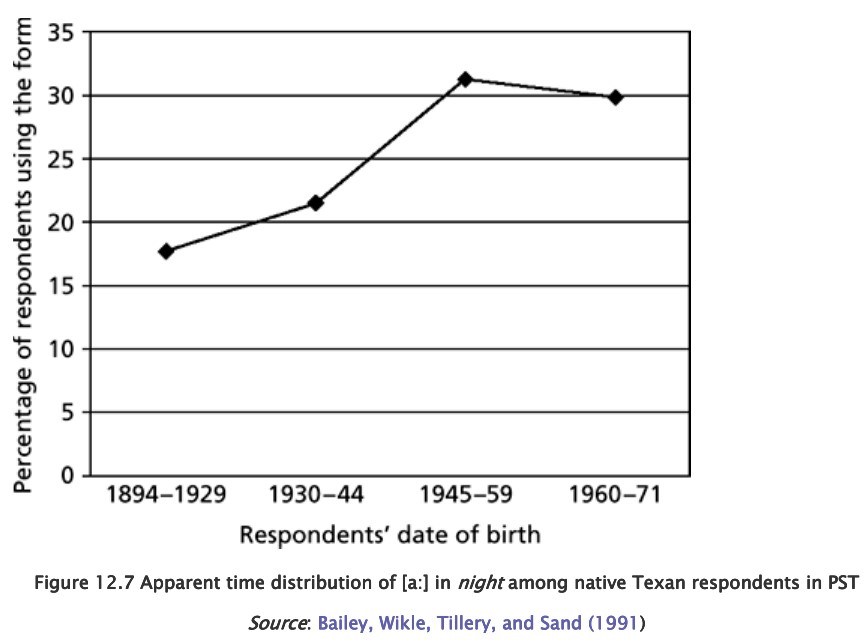
\includegraphics[scale=0.9]{texas_ai.jpg}

        The graph above presents data on the linguistic variable (aɪ) from speakers in Texas when they say the word \textit{night}, which can be realized as either the diphthong [aɪ] or the monophthong [aː]. Pay special attention to \emph{all} of the dates and answer the following questions.
        \question[1] How many ages are in \emph{each} range of ages that speakers were grouped under? \hrulefill
        \question[1] What percentage of speakers between the ages of 47 and 61 at the time of the survey realized (aɪ) as [aː]? \hrulefill
        \question[1] What percentage of speakers between the ages of 20 and 31 at the time of the survey realized (aɪ) as [aɪ]? \hrulefill
        \question[1] What general trend for (aɪ) does this data suggest to us? \hrulefill

        \hrulefill

        \hrulefill

        \parbox{0.5\linewidth}{
          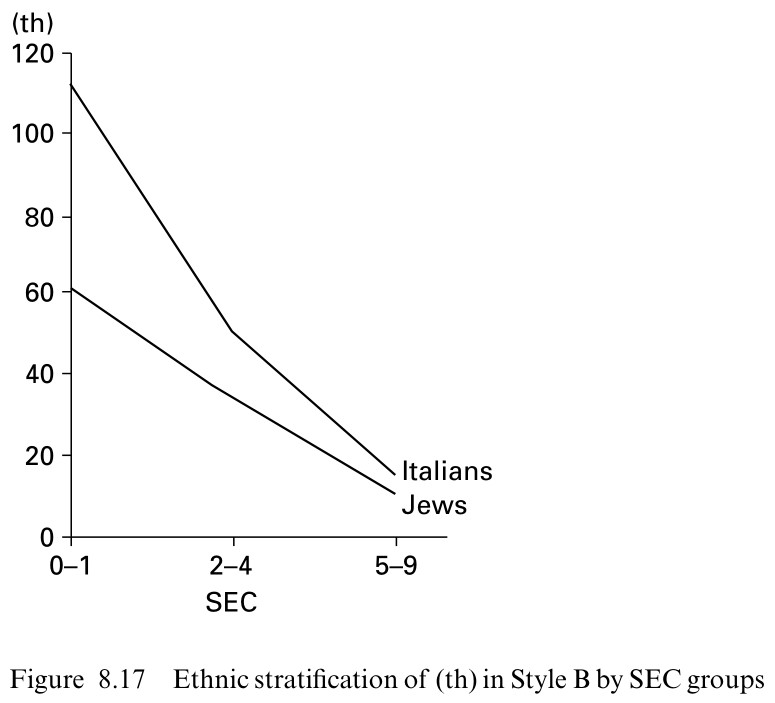
\includegraphics[scale=0.75]{ny_ethnicity_th.jpg}
        }
        \parbox{0.5\linewidth}{
          \fbox{\parbox{0.85\linewidth}{
          The graph on the left presents data on the linguistic variable (th) from speakers who were members of two different ethnic groups in the Lower East Side neighborhood of New York in the 1960s. This variable can be realized either as [t] or [θ]. The y-axis is an index where a higher values represent more [t] realizations and lower values represent more [θ] realizations. SEC stands for socio-economic class, where lower numbers represent lower-classes, middle numbers represent middle-classes, and higher numbers represent upper-classes.
          }}
        }
        \question[1] Looking only at the upper-classes, which ethnic group produced [t] more? \hrulefill
        \begin{parts}
          \part[1] What was the index of (th) for that group, roughly? \hrulefill
        \end{parts}
        \question[1] Did lower-class Jewish people or middle-class Italians produce [t] more? \hrulefill
        \question[1] Which ethnic group and socio-economic class combination produced [θ] the \emph{least}? \hrulefill
        \question[1] What was the overall trend for (th) from the lower-classes to the upper-classes? \hrulefill

        \hrulefill

        \hrulefill

    \newpage

    \section{Computational Linguistics}
      \instr{Use the text below, from the Brown corpus, to answer the following questions. When asked for parts-of-speech, simply give the abbreviations. You \emph{do not} need to know what the abbreviations stand for in order to complete this section. (1 point each)}
        \lstinputlisting[firstline=24, lastline=27]{../data/brown.txt}

        \question[1] What is the most frequent part-of-speech? \hrulefill
          \begin{parts}
            \part[1] How many types are there for this part-of-speech? \hrulefill
            \part[2] List any types that have more than one token, if any: \hrulefill

            \hrulefill
          \end{parts}
        \parbox{0.45\linewidth}{
          \question[1] How many types are there? \hrulefill
        }
        \hspace{0.1\linewidth}
        \parbox{0.45\linewidth}{
          \question[1] How many tokens are there? \hrulefill
        }

  \end{questions}

  \vspace{1.25cm}

  % Grade
  \begin{center}
    \gradetable[v][pages]
  \end{center}
\end{document}
